\documentclass[10pt]{sugconf-ish}
\usepackage[top=0.75in,bottom=0.875in,left=1in,right=1in]{geometry}
\usepackage{graphicx}

% ----- macro variables used by sugconf -----
\sugconfsubject{NESUG 2007}
\sugconfpapernumber{}
\sugconfkeywords{}


\title{ Handout For:\\Effective Forecast Visualization With SAS \SASregistered\\Detailed Instructions and Documentation}
\author{Samuel T. Croker,  Independent Consultant}
\usepackage[bookmarks=true,
  pdfauthor={\@author},
  pdfcreator={pdfLaTeX sugconf.cls},
  pdfkeywords={\SUGconfKeywords},
  pdfstartview=FitBH,
  pdfsubject={\SUGconfSubject},
  pdftitle={\@title}]{hyperref}


\usepackage{booktabs,nonfloat}
\usepackage{comment,color}


% ----- helpful new commands -----
\newcommand{\degs}{\ensuremath $^{\circ}$}
\newcommand{\mins}{\ensuremath $^{\prime}$}
\newcommand{\secs}{\ensuremath $^{\prime\prime}$}
\newcommand{\isDistr}{\ensuremath $\sim$ }
\newcommand{\xomment}[1]{\textcolor{red}{\textbf{#1}}}

\begin{document}
\section{Confidence Intervals as Regions}
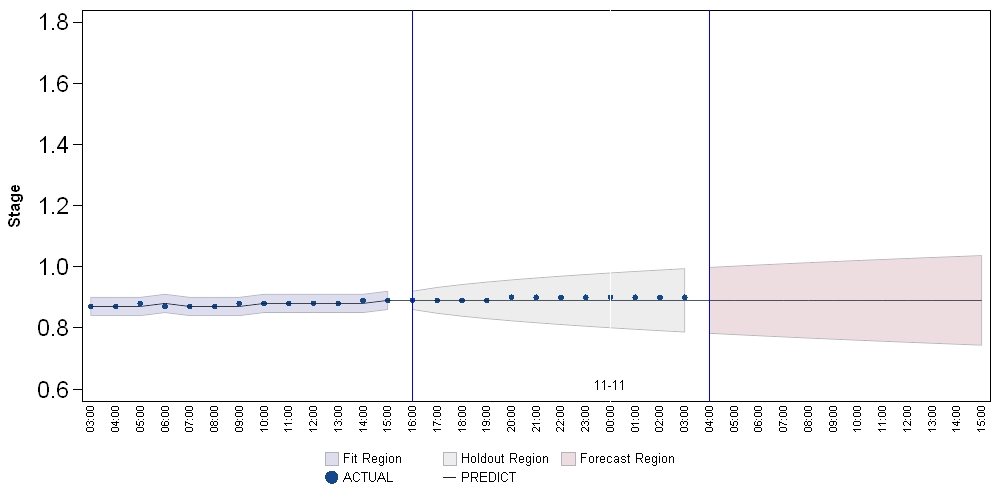
\includegraphics[width=6.5in]{3reg.jpg}\\
\includegraphics[width=4.5in]{layout.jpg}
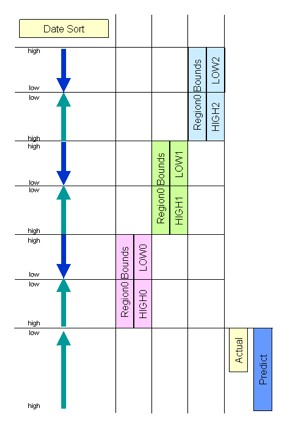
\includegraphics[height=3in]{ConfSort.jpg}

\section{SAS GRAPH Macro}
\scriptsize
\begin{verbatim}
/**********************************************************************

*   Program Name    :   $RCSfile: NP04.Handouts.tex,v $

*   REV/REV AUTH    :   $Revision: 1.1 $ $Author: scoyote $

*   REV DATE        :   $Date: 2008/03/23 15:37:37 $

***********************************************************************/ 

%macro threeregionforecast(

    /* positional parameters (required) */

     ds                   /* dataset containing forecasts */

    ,dataend              /* ending date of the time series - not the forecast series */

    ,datastart            /* starting date of the time series */

    ,plotback             /* how many date values to go back from the end of the series in the plot */

    ,predictlag           /* how many date values to predict ahead */

    /* optional parameters */

    ,order=                 /* date axis ordering (should be order=(<<data>>) )*/

    ,lciname=L95            /* variable name of the lower confidence bound */

    ,uciname=U95            /* variable name of the upper confidence bound */

    ,rsname=residual        /* variable name of the residual values */

    ,fcname=forecast        /* variable name of the forecast values */

    ,varname=actual         /* variable name of the actual values */

    ,varlab=                /* label for the actual values */

    ,fclab=                 /* label for the predict values */

    ,dtm=date               /* variable name of the date axis variable */

    ,dtdisplay=datetime28.  /* default format for the datetime axis */

    ,dtformat=mmddyy8.      /* format for time axis values */

    ,gname=FCST             /* name for the SAS graph output */

    ,gcat=work.GSEG         /* ouptut catalog */

    ,gdesc=Forecast Plot    /* description and title of the graph */

    ,fontname=SWISS         /* fonts */

    ,htitle=1               /* title height */

    ,cback=white            /* background color */

    ,grtitle=               /* main title of the graph */

    ,vaxisvalh=1            /* vertical axis value height */

    ,haxisvalh=1            /* horizontal axis value height */

    ,xinterval=hour.        /* order interval for the x axis */

    ,xminorticks=2

    ,ymajnum=10             /* number of y tick marks */

    ,hatitle=               /* horizontal axis title */

    ,vatitle=               /* vertical axis title */

    ,cicol1=bwh             /* first confidence region color */

    ,cicol2=gwh             /* second confidence region color */

    ,cicol3=pkwh            /* third confidence region color */

    /* the following apply to actual symbol values */        

    ,actcol=vigb            /* color */

    ,acth=1                 /* height */

    ,actw=1                 /* width */

    ,actv=dot               /* value type */

    ,actl=1                 /* line type */

    ,acti=none              /* interpolation type */

    /* the following apply to forecast symbol values */        

    ,fcstcol=degb           /* color */

    ,fcsth=1                /* height */

    ,fcstw=1                /* width */

    ,fcstl=1                /* line type */

    ,fcstv=none             /* value type */

    ,fcsti=j                /* interpolation type */

    );  

    data _null_;

        format forecaststart forecastend 20.;

        forecaststart=intnx('dthour',&dataend,-&plotback);

        forecastend=intnx('dthour',forecaststart,&predictlag);

        plotstart=intnx('dthour',forecaststart,-&plotback); 

        call symput ('forecaststart',forecaststart);

        call symput ('forecastend',forecastend);

        call symput ('plotstart',plotstart);

    run;

    /* rebuild the output data so that the cis plot as polygons */

    data out(  drop=     sval0 sval1 sval2)

            low0( keep=&dtm sval0 sval1 sval2)

            high0(keep=&dtm sval0 sval1 sval2)

            low1( keep=&dtm sval0 sval1 sval2)

            high1(keep=&dtm sval0 sval1 sval2)

            low2( keep=&dtm sval0 sval1 sval2)

            high2(keep=&dtm sval0 sval1 sval2);

        set &ds;

        where &dtm>=&plotstart;

        output out;

        if &dtm <= &forecaststart then do;

            sval0=&lciname; output low0; 

            sval0=&uciname; output high0;

        end;

        if &dtm > &forecaststart and &dtm <= &dataend then do; 

            sval1=&lciname; output low1; 

            sval1=&uciname; output high1; 

        end;

        if &dtm > &dataend then do; 

            sval2=&lciname; output low2; 

            sval2=&uciname; output high2;

        end;

    run;

    /* sort the lower bound datasets so that the polygons will be drawn correctly */

    proc sort data=low0; by descending &dtm; run;

    proc sort data=low1; by descending &dtm; run;

    proc sort data=low2; by descending &dtm; run;



    /* stack the low and high datasets in this way so that the graphs will be drawn correctly */

    data forecast; 

        set  

            low2 high2 

            low1 high1 

            low0 high0 

            out; 

        if &dtm=. then delete; 

    run;



    /* generate vertical lines to denote the date, and highlight the start of the different regions */

    data DayLines; set forecast(keep=&dtm );

        length color function $8 text $25;

        retain xsys '2' ysys '1' when 'a';

        if hour(&dtm)=0 and minute(&dtm)=0 and &dtm>=intnx('dthour',&plotstart,-1) then do;

            wdate=compress(day(datepart(&dtm))||'-'||month(datepart(&dtm)));

            function='move'; x=&dtm; y=0; 

                output;

            function='draw'; x=&dtm; 

                y=100; color='white'; size=1; output;

            function='label';x=&dtm; 

                y=3; size=1; position='2';  

                angle=90;color='black'; text=wdate; output;

        end;

        if &dtm=intnx('dthour',&forecaststart,1) 

            or &dtm=intnx('dthour',&dataend,1) then do;

            function='move';x=&dtm; y=0; output;

            function='draw';x=&dtm; y=100; color='blue'; size=1; output;

        end;

    run;





/* draw the graph */

    goptions reset=all

            device=activex 

            xpixels=1000

            ypixels=500 

            ftext="&fontname" 

            htitle=&htitle 

            cback=&cback  ;

    title &grtitle;

    symbol1 i=ms                                    c=&cicol1  co=libgr;

    symbol2 i=ms                                    c=&cicol2  co=libgr;

    symbol3 i=ms                                    c=&cicol3  co=libgr;

    symbol4 i=&acti  v=&actv    l=&actl  h=&acth    w=&actw    c=&actcol;

    symbol5 i=&fcsti v=&fcstv   l=&fcstl h=&fcsth   w=&fcstw   c=&fcstcol;

    legend1 across=10;

    title &grtitle;

    axis1 label=(&hatitle ) 

        value=(f="&fontname" h=&haxisvalh angle=90 rotate=0)  

        major=none

        minor=none

        order=(&plotstart to &forecastend by &xinterval);

    axis2 label=(&vatitle angle=90 rotate=0) 

        value=(h=&vaxisvalh) 

        minor=none;

    proc gplot data=forecast gout=work.gseg annotate=daylines;

        label sval0='Fit Region';

        label sval1='Holdout Region';

        label sval2='Forecast Region';

        label &varname=&varlab;

        label &fcname=&fclab;

        plot  sval0*&dtm=1 

        sval1*&dtm=2 

        sval2*&dtm=3 

        &varname*&dtm=4 

        &fcname*&dtm=5 

            /   name="&gname" des="&gdesc "

                grid

                haxis=axis1 

                vaxis=axis2 

                legend=legend1

                overlay 

                chref=palg;

        format &dtm &dtdisplay;

    run; quit;

%mend threeregionforecast;
\end{verbatim}
\section{ODS Graphics}
With ODS GRAPHICS, the plotting of confidence intervals as regions is much easier.
There is documentation for this type of work at \url{http://support.sas.com/rnd/base/topics/statgraph/proctemplate/a002774500.htm
} .\\
ODS Graphics can be accessed through many procedures, but can also be used (experimentally in 9.1.3) via the data step.  First a template must be declared.  There are many templates associated with procedures also, and these can be copied.  In the following example a template was created from scratch.
\scriptsize
\begin{verbatim}
ODS PATH work.templat(update) sashelp.templat(read) sashelp.tmplmst(read);

proc template;

    define statgraph mygraphs.stcfor;

    dynamic graphtit;

    layout lattice /width=900 height=200 border=false;

        layout overlay /border=false    

            xaxisopts=(display=(values TICKS) )

            yaxisopts=(display=all label="Stage" ) 

;

        entrytitle graphtit/

                fontsize=12

                fontweight=bold

                halign=left

                padtop=0

                padbottom=0

                valign=top;



            Band

                ylimitlower=fit_lower

                ylimitupper=fit_upper

                x=datestamp / 

                    fill=true 

                    lines=false 

                    fillcolor=ywh

                    legendlabel="Fit CI" 

                    name="Conf1";

            Band

                ylimitlower=holdout_lower

                ylimitupper=holdout_upper

                x=datestamp / 

                    fill=true 

                    lines=false 

                    fillcolor=bwh

                    legendlabel="Holdout CI" 

                    name="Conf2";

            Band

                ylimitlower=fcst_lower

                ylimitupper=fcst_upper

                x=datestamp / 

                    fill=true 

                    lines=false 

                    fillcolor=pkwh

                    legendlabel="Forecast CI" 

                    name="Conf3";

            scatter X=datestamp Y=actual  /name="act"  legendlabel="Actual Stage"  markers=true 
            		markersymbol=circlefilled markercolor=black ;

            SERIES X=datestamp Y=predict /name="pred" legendlabel="Predicted Stage" markers=false 					linecolor=blue;

        endlayout;

    endlayout;

    end;

run;
\end{verbatim}
\normalsize
A simple data step is used to plot the graph from ODS GRAPHICS.  The SQL statement shows how the limits for each forecast region are retrieved from the data.  The dataset \texttt{MARYLAND} contains the pre-forecasted data and \texttt{OUTFOR} contains the forecasts as generated by \texttt{HPFENGINE}.
\scriptsize
\begin{verbatim}

goptions reset=all;

ods html gpath='C:\Documents and Settings\scoyote\Desktop\Output';

ods graphics on /reset imagename="forecastplot" imagefmt=jpeg border=off;

    

    proc sql noprint;

        select 

               max(datestamp) format=30.

             , min(datestamp) format=30.

            into 

                :maxdt

                ,:mindt

            from maryland 

            where site_no="03078000";

    quit; 

    data _null_;

        merge outfor(

                    where=(site_no='03078000')

                    rename=(lower=low upper=up)

                    in=outfor)

              sitenames;

        by site_no;

        call symput('sitename',station_nm);

        if outfor;

        if datestamp<=intnx('hour',&maxdt,-&back) then do;

                fit_lower=low; fit_upper=up;

        end;

        else if datestamp<=&maxdt then do;

                holdout_lower=low; holdout_upper=up;

        end;

        else if datestamp>&maxdt then do;

                fcst_lower=low; fcst_upper=up;

        end;

        file print ods=( template='mygraphs.stcfor' 

            objectlabel='Forecast Plot' dynamic=(graphtit=station_nm) );

        put _ods_ ;

    run;

ods html close;

ods graphics off;
\end{verbatim}\normalsize

\begin{minipage}{\linewidth} 
\centering
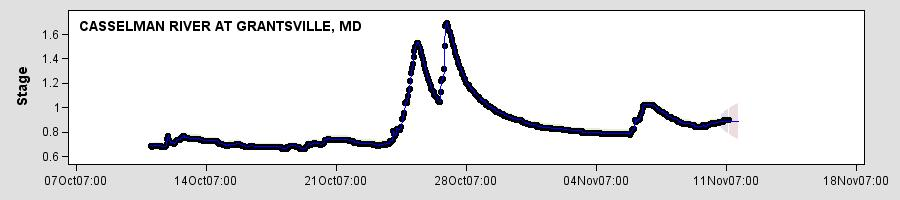
\includegraphics[width=6in,keepaspectratio]{forecastplot0.jpeg} 
\figcaption{Cassleman River Near Grantsville, MD October 7th--November 11th, 2007}
\label{fig:Cassleman1}
\end{minipage}\\
\begin{minipage}{\linewidth} 
\centering
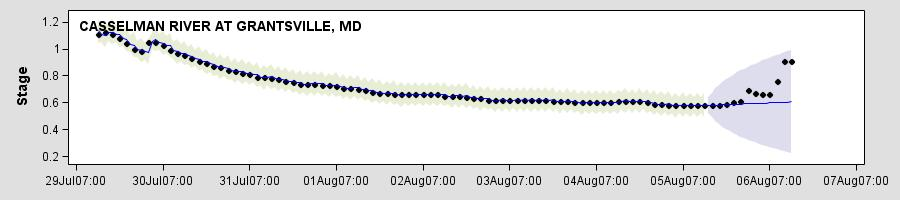
\includegraphics[width=6in,keepaspectratio]{03078000B24_L24_0.jpeg} 
\figcaption{Cassleman River Near Grantsville, MD August 5th--6th, 2007}
\label{fig:Cassleman2}
\end{minipage}\\
\begin{minipage}{\linewidth} 
\centering
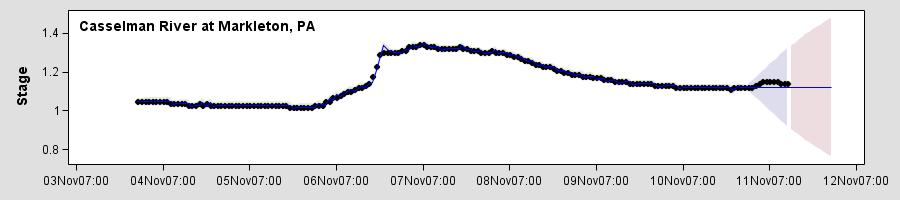
\includegraphics[width=6in,keepaspectratio]{03079000B12_L24_0.jpeg} 
\figcaption{Cassleman River Near Markleton, PA October 7th--November 11th, 2007}
\label{fig:Cassleman3}
\end{minipage}

\newpage
\section{Sparklines}
\subsection{Small Stacked Graphics}
The following graphs are easily comparable without too much detail information that could be included in many different ways, such as a drill down.\\

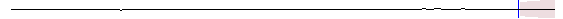
\includegraphics{fc01581920.pdf}Gunpowder Falls near Parkton, MD\\
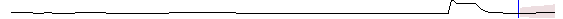
\includegraphics{fc01582000.pdf}Little Falls at Blue Mount, MD\\
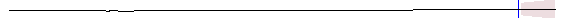
\includegraphics{fc01591000.pdf}Patuxent River near Unity, MD\\
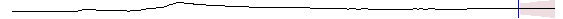
\includegraphics{fc01595000.pdf}North Branch Potomac River at Steyer, MD\\
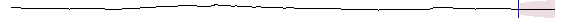
\includegraphics{fc01596500.pdf}Savage River near Barton, MD\\
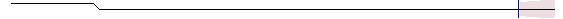
\includegraphics{fc01597500.pdf}Savage River below Savage River Dam \\
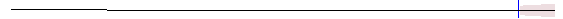
\includegraphics{fc01598500.pdf}North Branch Potomac River at Luke, MD\\
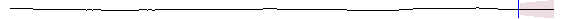
\includegraphics{fc01609000.pdf}Town Creek near Oldtown, MD\\
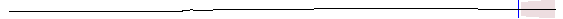
\includegraphics{fc01649150.pdf}Paint Branch Tributary near Colesville, MD\\
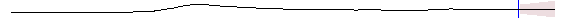
\includegraphics{fc03075500.pdf}Youghiogheny River near Oakland, MD\\
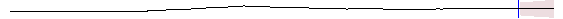
\includegraphics{fc03076500.pdf}Youghiogheny River at Friendsville, MD\\
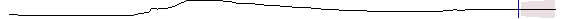
\includegraphics{fc03078000.pdf}Casselman River at Grantsville, MD\\
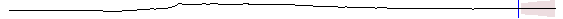
\includegraphics{fc03079000.pdf}Casselman River at Markleton, PA\\

\includegraphics{spark_axis.pdf}


These graphics can also be used in the flow of the text if formatted correctly.  The SASHELP.AIR series is shown 
\includegraphics{Croker_airlineminmax.pdf} flowing with the text.  The code to generate this sparkline is shown below, and is an example of how to use inline sizing options in the GOPTIONS statement:
\scriptsize
\begin{verbatim}
filename outgraph "path.file"; 

goptions  

     reset=all 

     device=pdfc

     xmax=144pt  horigin=0.000pt  hsize=144pt xpixels=5000

     ymax=12pt   vorigin=0.000pt  vsize=12pt  ypixels=416

     cback=white

     noborder

     gsfname=outgraph

     gsfmode=replace;

     symbol1 v=none i=j c=black width=50;

     axis1 label=none value=none major=none minor=none 

 offset=(0,0)

 style=0; 

     axis2 label=none value=none major=none minor=none

 style=0;

proc sql noprint;

     select min(air)

          , max(air)    

           into 

                 :minair 

               , :maxair

     from sashelp.air;

quit;

data air;

     set sashelp.air;

     if air=&maxair then maxair=air;

     if air=&minair then minair=air;

run;

symbol2 v=dot h=40 c=red i=none;

symbol3 v=dot h=40 c=green i=none;



proc gplot data=air;

     plot (air maxair minair)*date / overlay   haxis=axis1 vaxis=axis2;run;

quit;

\end{verbatim}\normalsize

\newpage
\section{Example - Time Series Diagnostics}
\subsection{Long Period Correlations - 768 Lags}
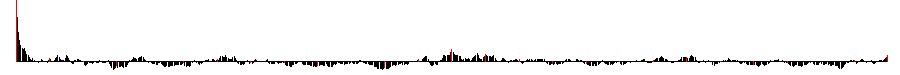
\includegraphics{spark_corr_id_.pdf} ACF\\
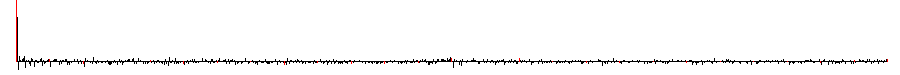
\includegraphics{spark_partcorr_id_.pdf} PACF\\
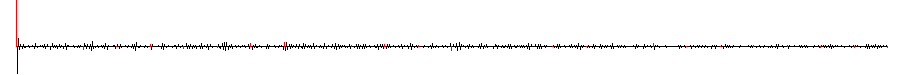
\includegraphics{spark_invcorr_id_.pdf} IACF\\

\subsection{Short Period Correlations }

\includegraphics{spark_corr_id_zoom.pdf} ACF\\

\includegraphics{spark_partcorr_id_zoom.pdf} PACF\\

\includegraphics{spark_invcorr_id_zoom.pdf} IACF\\

\subsection{Comparative Boxplots}
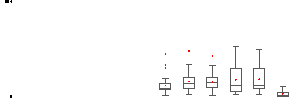
\includegraphics{sparkbox_actual2002}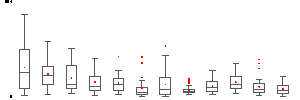
\includegraphics{sparkbox_actual2003}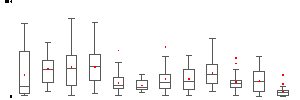
\includegraphics{sparkbox_actual2004}\\
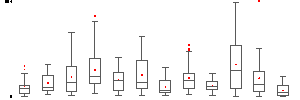
\includegraphics{sparkbox_actual2005}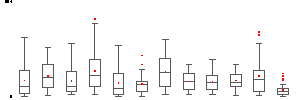
\includegraphics{sparkbox_actual2006}
\includegraphics{sparkbox_actual2007}\\

\subsection{$\chi^2$ Probabilities}

\includegraphics{spark_probchisq_id_.pdf} Series\\

\includegraphics{spark_probchisq_res_.pdf} Residual\\

\subsection{Time Series}

\includegraphics{spark_demand02.pdf}\\
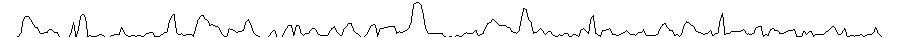
\includegraphics{spark_demand03.pdf}\\

\includegraphics{spark_demand04.pdf}\\

\includegraphics{spark_demand05.pdf}\\

\includegraphics{spark_demand06.pdf}\\

\includegraphics{spark_demand07.pdf}\\

\includegraphics{spark_zero_axis.pdf}\\

\newpage
\section{References}

\begin{list}{}{\setlength{\leftmargin}{2em}\setlength{\itemindent}{0em}\raggedright}
\item Tufte, Edward R. 2006. 
\emph{Beautiful Evidence},  Cheshire, CT: Graphics Press LLC.

\item Gossens, Michael, Frank Mittlebach, Alexander Samarin \emph{The \LaTeX Companion}, 1st Edition : Addison-Wesley Professional

\item Box, George E.P., Gwilym M. Jenkins and Gregory C. Reinsel. 1994. 
\emph{Time Series Analysis: Forecasting and Control}, 3rd ed. Upper Saddle River, NJ: Prentice-Hall.

\item Brocklebank, John and David A. Dickey. 2003. 
\emph{\SASregistered\ for Forecasting Time Series}, 2nd ed. Cary, NC: SAS Institute Inc.

\item Gelso, Charlie, Larry Coburn. 2006. \emph{Guide to Maryland Trout Fishing:  The Catch and Release Streams} Carter, OK: Falling Star Publishing

\item Cartier, Jeff. ``The Power of the Graphics Template Language.'' \emph{Proceedings of the 30th Annual \SASregistered\ Users Group International Conference}. April 2004. %\\
$<$\url{http://support.sas.com/rnd/datavisualization/papers/sugi30/GTL.pdf}$>$ (Accessed July 18, 2007).

\item Croker, Samuel T. ``Effective Forecast Visualization with SAS/GRAPH.'' \emph{SAS Global Forum 2007 Proceedings}. April 2007. \\ $<$\url{http://www8.sas.com/scholars/Proceedings/2006/DataPresentation/DP01_06.PDF}$>$

\item SAS Institute Inc.\emph{ Sample 1151: Filling the area between plot lines using SYMBOL statement} \\ $<$\url{http://support.sas.com/ctx/samples/index.jsp?sid=115}$>$

\item SAS Institute Inc.\emph{ARIMA: Models for Series J from Box-Jenkins}\\$<$\url{http://ftp.sas.com/techsup/download/sample/samp_lib/etssampArima_Models_for_Series_J_from_B.html}$>$


\item Shumway, Robert H. and David S. Stoffer. 2006. 
\emph{Time Series Analysis and Its Applications with R Examples}, 2nd ed. New York: Springer Science+Business Media, LLC.
\end{list}




%\section{Acknowledgments}



\newpage
\section{Contact Information}
We value and encourage your comments and questions! You can find the latest version of the SAS code for this paper at: \url{http://www.scoyote.net/forecasting/}. Please note that we may update this code for use in other papers.

You can contact the authors at:

\begin{tabular}[t]{rl}
\textbf{Name:} & Samuel T. Croker \\
%\textbf{Address:} & Kyzer Rd \\
% & Lexington, SC 29073 \\
%Work Phone:        & 803-240-2805 \\
%Fax:               & 987-654-3210                     \\
%\textbf{E-Mail:} & \href{scoyote@scoyote.net?subject=SESUG 2007 Paper Question}
%{\texttt{scoyote@scoyote.net}} \\
\textbf{E-Mail:} & \texttt{scoyote at scoyote.net} \\
\textbf{Web:} & \url{http://www.scoyote.net/forecasting/} \\
 \end{tabular}


\vfill
% ----- macro variables used by sugconf -----
\SASisRegisteredTrademark\ \OtherTrademarks


\end{document}
